\section{Myonische Fusion}

\begin{frame}{Myonenkatalysierte Fusion}
    \begin{columns}
        \begin{column}{0.55\textwidth}
            \begin{itemize}
                \item<+-> \textbf{Myon}:
                \begin{itemize}
                    \item Ladung: $q_\mu = -1\,e$
                    \item Masse: $m_\mu = 206.768\,m_\text{e}$
                    \item Lebensdauer: $\SI{2.197e-6}{\s}$ \\
                     (Zerfällt: $\mu^- \to e^- + \overline{\nu}_e + \nu_\mu$)
                    \item Spin: $s= \frac{1}{2}$
                \end{itemize}
                \item<+-> In H/D/T-Atom oder $\text{H/D/T}_2$ kann Myon die Elektronen verdrängen
                \item<+-> ähnliche Orbitale aus wie $e^-$ Atome, aber mit vielfach geringerer räumlicher Ausdehnung
                \item<+-> Kerne kommen sich näher daher Fusion bei viel niedrigeren Temperaturen möglich
                \item<+-> Bei Fusion wird Myon wieder frei
                \item<+-> Theoretisch vorhergesagt 1947 \cite{myonTheory} und nachgewiesen 1957 \cite{myonExp}
            \end{itemize}
        \end{column}
        \begin{column}{0.45\textwidth}
            \begin{center}
                \only<2->{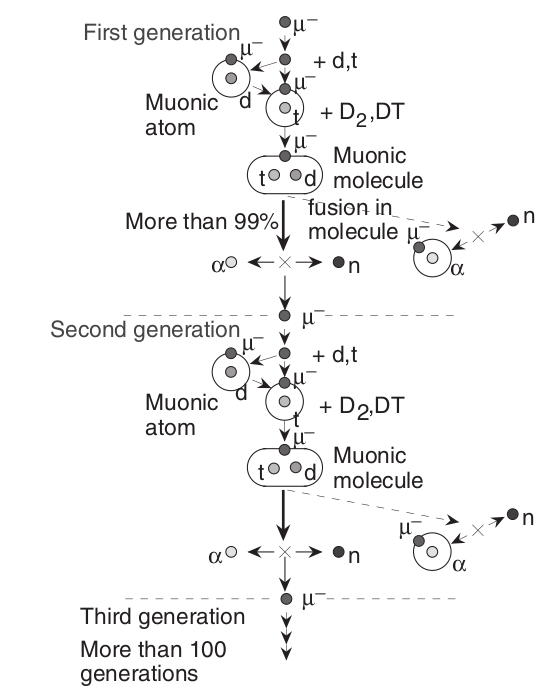
\includegraphics[width=0.9\textwidth]{images/FusionCyclus.png}
                \small{Myonischer Fusionszyklus \cite[S.71]{Naga03}}}
            \end{center}
        \end{column}
    \end{columns}
\end{frame}

\begin{frame}{Tunnelwahrscheinlichkeiten}
    \centering
    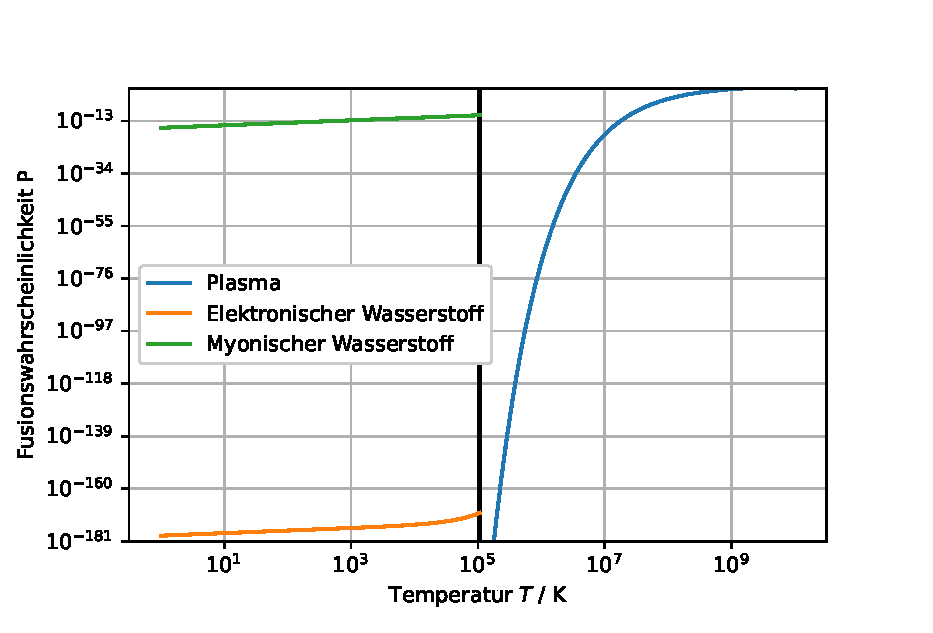
\includegraphics[width=0.8\textwidth]{images/Tunnelwahrscheinlichkeiten.eps}
\end{frame}

\begin{frame}{Energiebilanz}
    \begin{itemize}
        \item<+-> Produktion von Myonen im Teilchenbeschleuniger (z.B. $S\mu S$ Methode)
        \item<+-> Protonen werden auf C-Atome geschossen, dabei entstehen Pionen, die in Myonen zerfallen
        \item<+-> Energieaufwand im besten Fall: $\SI{-5}{\giga\eV}$ pro Myon \cite[S.93]{Naga03}
        \item<+-> Unter Vernachlässigung aller Verluste beim Transport, o.a. kann jedes Myon in etwa 150 Fusionen ermöglichen \cite[S.97]{Naga03}, bis sie
        \begin{itemize}
            \item durch Zerfall verloren gehen
            \item an ein Fusionsprodukt gebunden werden
        \end{itemize}
        \item<+-> Je nach Fusionsprozess werden zwischen $\SI{3.3}{\mega\eV}$ und $\SI{24}{\mega\eV}$ frei
        \item<+-> Energiegewinn: $\SI{3.6}{\giga\eV}$ pro Myon (für \SI{24}{\mega\eV}) \\ $\Rightarrow$ Netto Energieverbrauch
        \item<+-> Für Nutzbarkeit zur Stromerzeugung wäre ein Energiegewinn von etwa $\SI{20}{\giga\eV}$ nötig
        \item<+-> Verbesserung: Verringerung der Erzeugungsenergie der Myonen, mehr Fusionen pro Myon ermöglichen
    \end{itemize}
\end{frame}

\section{Weitere Katalysatoren}

\begin{frame}{Weitere Katalysatoren}
    \begin{itemize}
        \item<+-> \textbf{Pyrofusion:} Ionisation und Beschleunigung von Deuteriumkernen mit pyroelektrischem Kristall als Spannungsquelle. Erzeugt 400-fache der natürlichen Neutronenstrahlung. Vermutete Ursache $\mathrm{D + D} \to \ ^3\mathrm{He} + \mathrm{n}$. \\
        \underline{Aber:} Beschränkung auf geringe Teilchenströme, daher nur als Neutronenquelle nutzbar und für Energieerzeugung ungeeignet. \cite{wiki:ColdFuison}
        \item<+-> \textbf{Sonofusion:} kontrollierte Fusion durch Erzeugung von Kavitation mit Schallwellen (Science-Artikel) \\
        \underline{Aber:} Gefälschte Ergebnisse (Bubblegate) \cite{FAZ}
        \item<+-> weitere dubiose Aufbauten bei denen eine genauere Überprüfung durch dritte verweigert wurde
    \end{itemize}
\end{frame}